\section{GumboNode}
\label{section:gumbo_node}

\begin{figure}[h!]
  \centering
  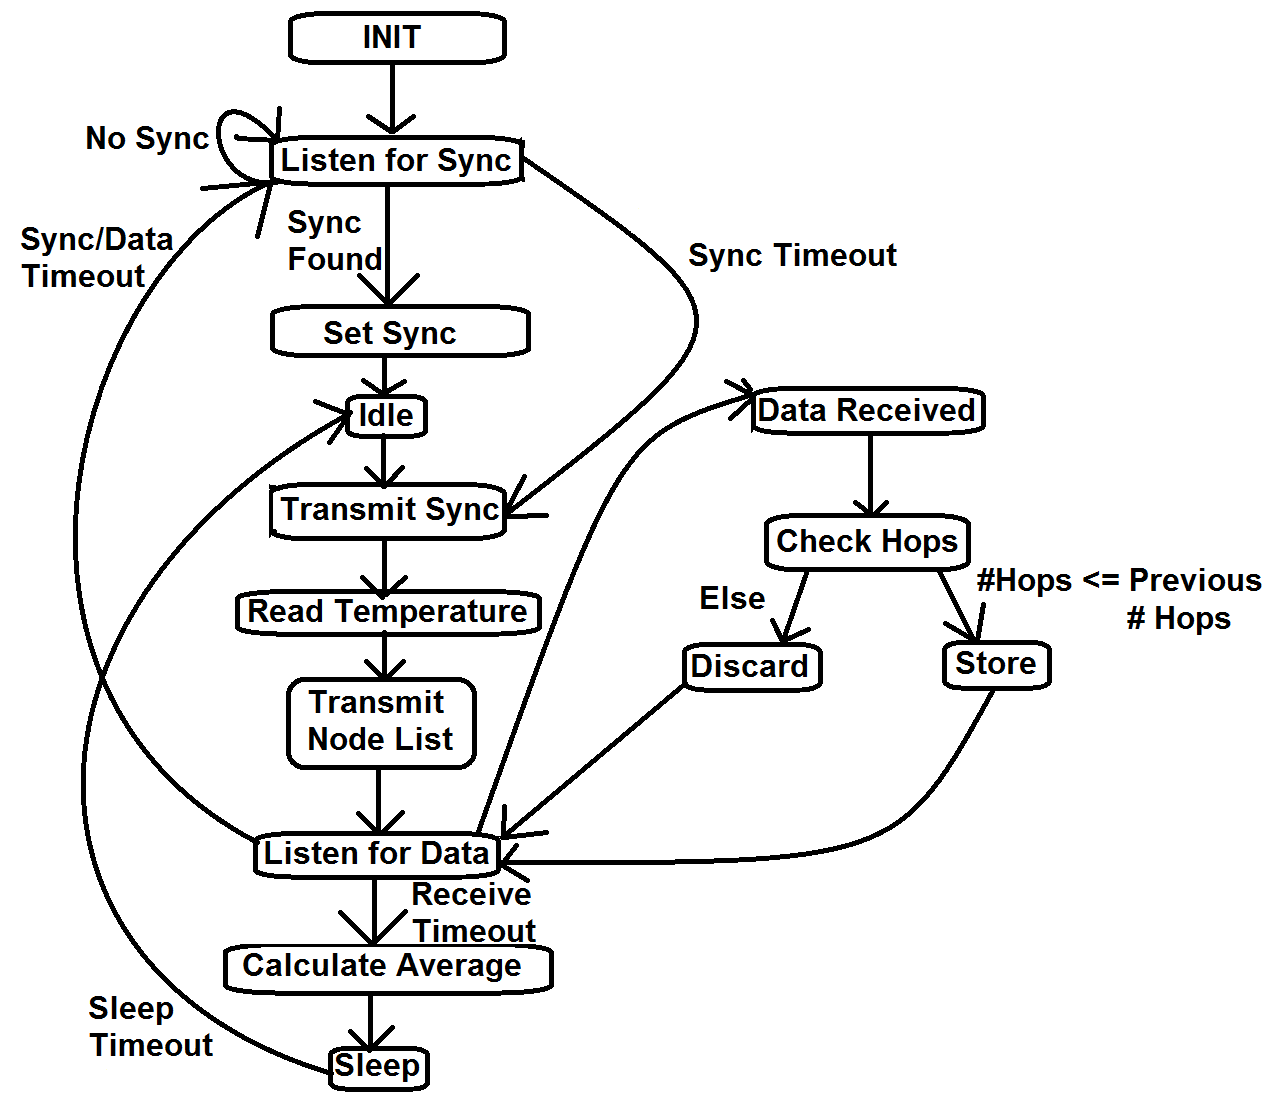
\includegraphics[width=0.5\textwidth]{images/algorithm_flowchart.png}
  \caption{A flowchart of the communication protocol.
  \label{img:flowchart}
  }
\end{figure}

\begin{figure}[h!]
  \centering
  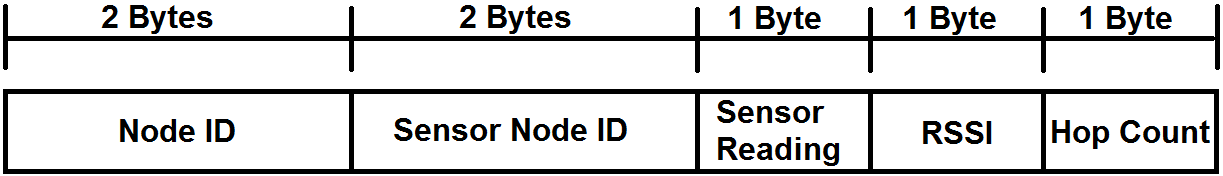
\includegraphics[width=0.5\textwidth]{images/packet_structure.png}
  \caption{Sensor packet list structure.
  \label{img:flowchart}
  }
\end{figure}

In order to accuratly profile the network, we have created minimum-cost hardware nodes to test the protocols on, which we have named
\textbf{GumboNodes}.  GumboNodes are barebones sensor nodes consisting of a microcontroller, a wireless transceiver, a sensor, and a battery. In our specific hardware, the system already comes on-board with a temperature sensor. 

We selected the ATTiny85 as the microcontroller for the chip. The ATTiny85 is a low-cost, low-power 8-bit processor. It is Arduino-compatible and has a wide range of options to optimize the processor for power consumption. Table 1 provides power information from the datasheet [6]. In the lowest power mode, the processor uses less than 2 μA. There are only two ways to wake the chip from this deep sleep: an external interrupt caused by a logic level change on an input pin, or periodically by an internal oscillator known as the watchdog timer. The watchdog timer has maximum time limit of 8 seconds after which the microcontroller automatically wakes up and enters idle state. The system may immediately be put back to sleep, or act after it wakes up a certain number of times.

The Texas Instruments CC2500 was selected as the wireless chip. The CC2500 is a low-level 2.4GHz wireless transceiver. Communication occurs over a 4-wire serial perhiperal interface (SPI) [7]. The ATTiny85 we selected lacks an onboard SPI interface, but has a universal serial interface (USI) that is capable of interfacing with the transceiver. The CC2500 also has a temperature sensor on-board, which served as our sensor. 

A flowchart of the node’s behavior is provided in Figure 1. After power-on, the system immediately goes into receive mode.
